\documentclass[12pt]{article}
%\usepackage[pass,letterpaper]{geometry}              %This package needs to be enaled when dvi--->ps----->PDF
\usepackage{stmaryrd, amsfonts, mathptmx, mathtools, array, siunitx, subfigure, graphicx, listings, etoolbox, mdwlist }
\usepackage{multirow, indentfirst, cite, verbatim, keyval, textcomp, enumerate, calc, microtype, color,marvosym}

\usepackage[colorlinks,linktocpage,dvips]{hyperref}
\hypersetup{
   colorlinks   = true,                               %Colours links instead of ugly boxes
   urlcolor     = blue,                               %Colour for external hyper links
   linkcolor    = blue,                               %Colour of internal links
   citecolor    = red,                                %Colour of citations
   setpagesize  = false,
   linktocpage  = true,
}

\makeatletter
\patchcmd{\l@section}
  {\hfil}
  {\leaders\hbox{\normalfont$\m@th\mkern \@dotsep mu\hbox{.}\mkern \@dotsep mu$}\hfill}
  {}{}
\makeatother
\definecolor{anti-flashwhite}{rgb}{0.95, 0.95, 0.96}
\lstset{
backgroundcolor=\color{anti-flashwhite},
basicstyle=\small\ttfamily,
columns=flexible,
breaklines=true
}


\newcommand{\shellcmd}[1]{\\\indent\indent\texttt{\footnotesize\$ #1}\\}
\parskip 0.5em
\parindent 2em
\setlength{\textwidth}{6.0in} \setlength{\textheight}{8.8in}
\setlength{\topmargin}{0.4in} \setlength{\headheight}{0.0in}
\setlength{\headsep}{0.0in} \setlength{\oddsidemargin}{0.25in}
\setlength{\parindent}{.2in}
%\renewcommand{\baselinestretch}{1.5}
\setlength{\parindent}{2em}
\setlength{\parskip}{1em}
%%%%%%%%%%%%%%%%%%%%%%%%%%%%%%%%%%%%%%%%%%%%%%%%%%%%%%%%%%%%%%%%%%%%%%%%%%%
\title{\textbf{INSTALLATION GUIDE FOR TORCH}\\\textbf{THEANO, TENSORFLOW, CAFFE AND R}\\ \textbf{WITH CPU AND GPU}}%

\author{Data Science Program, GWU, USA \\
School of Electrical and Computer Engineering, OSU, USA\\
\vspace{1cm}\\
\Letter : martin.t.hagan@okstate.edu\\
\Letter : ajafari@gwu.edu\\
\Letter : amir.h.jafari@okstate.edu  }
%%%%%%%%%%%%%%%%%%%%%%%%%%%%%%%%%%%%%%%%%%%%%%%%%%%%%%%%%%%%%%%%%%%%%%%%%%%
\begin{document}
\begin{figure}
\centering 
\includegraphics[width=2in, height=1in]{fig/GW_logo.eps}\hfill
\centering 
\includegraphics[width=1in, height=1in]{fig/logo1.eps}\hfill
\end{figure}

%%%%%%%%%%%%%%%%%%%%%%%%%%%%%%%%%%%%%%%%%%%%%%%%%%%%%%%%%%%%%%%%%%%%%%%%%%%
\maketitle
\newpage
\tableofcontents
\newpage
\listoffigures
\newpage
%\listoftables
% \newpage
%\lstlistoflistings
% \newpage
%%%%%%%%%%%%%%%%%%%%%%%%%%%%%%%%%%%%%%%%%%%%%%%%%%%%%%%%%%%%%%%%%%%%%%%%%%%
\section{UBUNTU 14.04 DUAL BOOT INSTALLATION}

To boot from USB, will have to choose boot from USB option from within Windows itself. Either with PC Setting (bios setting) and change the boot sequence to USB.
\begin{figure}[h]
\centering 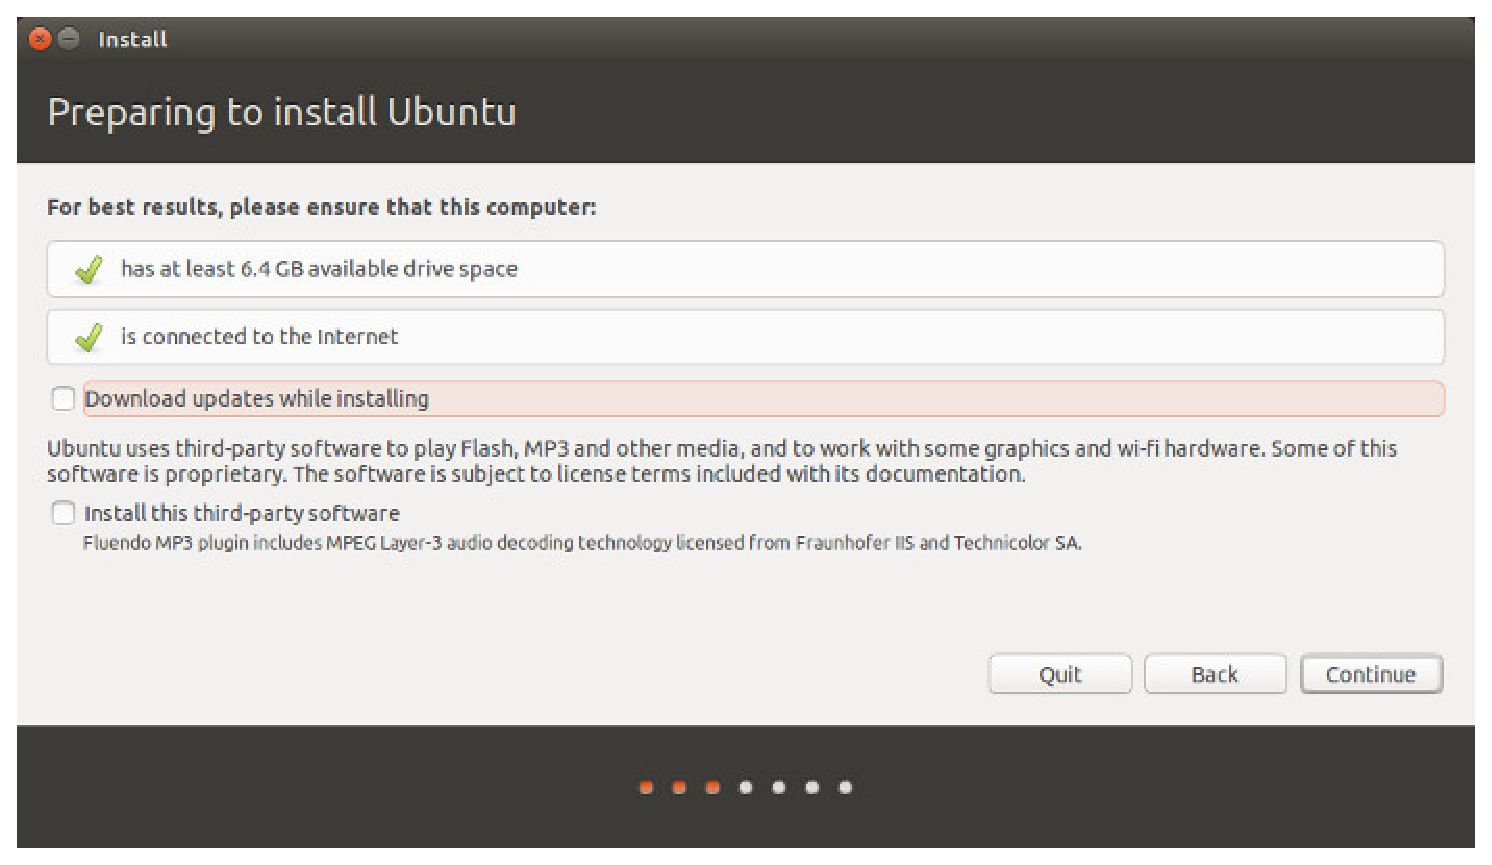
\includegraphics[width=5.8in, height=2.5in]{fig/d1.eps}
\caption{Space allocation}
\end{figure}b

Once you have booted in the live USB, you will be presented with option to try or install Ubuntu. Click on install. You will be presented with few screen options to choose the language. It will then do some checks on available space, power and internet connection etc. \textbf{Just click on Continue}. \textbf{Note, do not change the partition size}.
\begin{figure}[h]
\centering \includegraphics[width=5.8in, height=3in]{fig/d2.eps}
\caption{Automatic partition}
\end{figure}

\newpage
%%%%%%%%%%%%%%%%%%%%%%%%%%%%%%%%%%%%%%%%%%%%%%%%%%%%%%%%%%%%%%%%%%%%%%%%%%%


\section{NVIDIA AND CUDA 7.5 INSTALLATION}

\textbf{Installing CUDA Toolkit 7.5 on Ubuntu 14.04 Linux}

The following explains how to install CUDA Toolkit 7.5 on 64-bit Ubuntu 14.04 Linux. I have tested it on a self-assembled desktop with NVIDIA GeForce GTX Black Titan graphics card. The instruction assumes you have the necessary CUDA compatible hardware support. Depending on your system configuration, your mileage may vary \cite{NVIDIADRIVER}.

\textbf{CUDA Repository Download}
\begin{enumerate}
  \item Retrieve the CUDA repository package for Ubuntu 14.04 from the provided file.
  \item Put run file in the following directory (\textbackslash home \textbackslash Downloads)
   \item Search for terminal, put on to task bar, and open it (then do the following commands).
\suspend{enumerate}

\begin{lstlisting}
    $ cd \Downloads

    $ ls
\end{lstlisting}

\resume{enumerate}
    \item You should be able to see cuda\_7.5.18\_linux.run
\suspend{enumerate}

\textbf{CUDA Toolkit and Display Driver Installation}

\resume{enumerate}
    \item Then you have to kill the xserver by entering the following command into terminal.
\suspend{enumerate}

\begin{lstlisting}
    $ sudo service lightdm stop
\end{lstlisting}

\resume{enumerate}
    \item The gui will switch off and you will see the black screen.
    \item Hold the Ctrl+Alt+F1 key.
    \item Type in username and hit enter.
    \item Type in password (you will not see what you type in.)
    \item Enter the following commands.
    \item \textbf{Note: Any time you copy and paste underscore go back and replace it with new underscore in terminal.}
\suspend{enumerate}

\begin{lstlisting}
    $ cd \Downloads

    $ ls

    $ chmod +x cuda_7.5.18_linux.run
\end{lstlisting}

\resume{enumerate}
    \item Start the installation by the following command.
    \item \textbf{Note: Any time you copy and paste underscore go back and replace it with new underscore in terminal.}
\suspend{enumerate}

\begin{lstlisting}
    $./cuda_7.5.18_linux.run
\end{lstlisting}

\resume{enumerate}
\item Press q key to skip the read me file.
\item accept EULA ------ accept.
\item when terminal prompts for yes or no always yes.
\item when terminal asks for location hit enter (this is the default location)
\item after the the installation finished, we need to reboot. Do the following commands to reboot.
\suspend{enumerate}

\begin{lstlisting}
    $ sudo su

    # reboot
\end{lstlisting}

\resume{enumerate}
\item Redo the steps from 9 to 24 again for the full installation \textbf{except} for the following command.
\end{enumerate}

\begin{lstlisting}
    $ chmod +x cuda_7.5.18_linux.run
\end{lstlisting}

Now, after the system is rebooted you can search the additional driver in the Linux search box (first item in the taskbar) and you should be able to see the manually install driver checked. Also you can see check this command to be sure the GPU is installed correctly.

This following command checks to see if the installation worked properly.

\begin{lstlisting}
    $ nvidia-smi
\end{lstlisting}

\newpage
%%%%%%%%%%%%%%%%%%%%%%%%%%%%%%%%%%%%%%%%%%%%%%%%%%%%%%%%%%%%%%%%%%%%%%%%%%%
\section{TORCH INSTALLATION GUIDE}

\begin{enumerate}
    \item Torch can be installed to your home folder in {\tiny $\sim$}/torch by running these three commands \cite{TORCH}:
    \item Open terminal and enter the following commands.
    \item \textbf{Note: Any time you see yes or no in the installation type yes}.
\suspend{enumerate}

\begin{lstlisting}
    $ sudo apt-get install git

    $ git clone https://github.com/torch/distro.git ~/torch --recursive

    $ cd ~/torch; bash install-deps;

    $ cd ~/torch

    $ ./install.sh
\end{lstlisting}

\resume{enumerate}
    \item The first script installs the basic package dependencies that LuaJIT and Torch require. The second script installs LuaJIT, LuaRocks, and then uses LuaRocks (the lua package manager) to install core packages like torch, nn and paths, as well as a few other packages.

    \item The script adds torch to your PATH variable. You just have to source it once to refresh your env variables. The installation script will detect what is your current shell and modify the path in the correct configuration file.
    \item Enter the following command.
\suspend{enumerate}

\begin{lstlisting}
    $ cd ..

    $ source ~/.bashrc
\end{lstlisting}

\resume{enumerate}
    \item New packages can be installed using Luarocks from the command-line:
\end{enumerate}

\begin{lstlisting}

    $ sudo apt-get install luarocks

    $ luarocks install image

    $ luarocks list

    $ luarocks install nngraph

    $ luarocks install optim

    $ luarocks install nn

    $ luarocks install cutorch

    $ luarocks install cunn

\end{lstlisting}

\textbf{\emph{Now, it is time to test TORCH and check the installation, follow the instruction on Section \ref{TEST TORCH}.}}

\newpage
%%%%%%%%%%%%%%%%%%%%%%%%%%%%%%%%%%%%%%%%%%%%%%%%%%%%%%%%%%%%%%%%%%%%%%%%%%%
\section{cuDNN INSTALLATION GUIDE}

\begin{enumerate}
  \item Retrieve the cuDNN repository package for Ubuntu 14.04 from the provided file.
  \item Copy the file to Downloads folder. Then open terminal
  \item \textbf{Note: If the command wraps to another line highlight the first line then paste to terminal and then repeat for the next line then hit enter.}
\end{enumerate}

Uncompress and copy the cuDNN files into the toolkit directory. Assuming the toolkit is installed in /usr/local/cuda, run the following commands (edited to reflect the cuDNN version you downloaded)\cite{cuDNN}:

\begin{lstlisting}

    $ cd \Downloads

    $ tar xvzf cudnn-7.5-linux-x64-v5.0-ga.tgz

    $ sudo cp cuda/include/cudnn.h /usr/local/cuda/include

    $ sudo cp cuda/lib64/libcudnn* /usr/local/cuda/lib64

    $ sudo chmod a+r /usr/local/cuda/include/cudnn.h /usr/local/cuda/lib64/libcudnn*

\end{lstlisting}

\newpage
%%%%%%%%%%%%%%%%%%%%%%%%%%%%%%%%%%%%%%%%%%%%%%%%%%%%%%%%%%%%%%%%%%%%%%%%%%%
\section{THENAO INSTALLATION GUIDE}

\begin{enumerate}
    \item For installing Theano and Phyton, open terminal and run the following commands.
    \item \textbf{Note: the first command there is a space between first line and second line.}
    \item \textbf{Note: Any time you see yes or no in the installation type yes}.
\end{enumerate}

\begin{lstlisting}
    $ sudo apt-get install python-numpy python-scipy python-dev python-pip python-nose g++ libopenblas-dev git

    $ sudo pip install Theano
\end{lstlisting}

\textbf{\emph{Now, it is time to test THEANO and check the installation, follow the instruction on Section \ref{TEST THEANO}.}}

\newpage
%%%%%%%%%%%%%%%%%%%%%%%%%%%%%%%%%%%%%%%%%%%%%%%%%%%%%%%%%%%%%%%%%%%%%%%%%%%
\section{TENSORFLOW INSTALLATION GUIDE}

\textbf{Pip Installation}

\begin{enumerate}
  \item Pip is a package management system used to install and manage software packages written in Python. The packages that will be installed or upgraded during the pip install are listed in the REQUIRED\_PACKAGES section of setup.py \cite{TENSORFLOW}.
  \item Open terminal and try the following commands to install TensorFlow.
  \item \textbf{Note: Any time you copy and paste underscore go back and replace it with new underscore in terminal (the last command contains underscores).}
\end{enumerate}


\begin{lstlisting}
    $ sudo apt-get install python-pip python-dev

    $ export TF_BINARY_URL=https://storage.googleapis.com/tensorflow/linux/cpu/tensorflow-0.10.0rc0-cp27-none-linux_x86_64.whl

    $ export TF_BINARY_URL=https://storage.googleapis.com/tensorflow/linux/gpu/tensorflow-0.10.0rc0-cp27-none-linux_x86_64.whl

    $ sudo pip install --upgrade $TF_BINARY_URL
\end{lstlisting}

\textbf{\emph{Now, it is time to test TENSORFLOW and check the installation, follow the instruction on Section \ref{TEST TENSORFLOW}.}}

\newpage
%%%%%%%%%%%%%%%%%%%%%%%%%%%%%%%%%%%%%%%%%%%%%%%%%%%%%%%%%%%%%%%%%%%%%%%%%%%
\section{CAFFE INSTALLATION GUIDE}

\begin{enumerate}
  \item First, we need to install general dependencies by running the following commands \cite{CAFFE}.
  \item Open terminal.
  \item \textbf{Note: Any time you see yes or no in the installation type yes}.
  \item \textbf{Note: the first command there is a space between first line and second line.}
\suspend{enumerate}

\begin{lstlisting}
    $ sudo apt-get install libprotobuf-dev libleveldb-dev libsnappy-dev libopencv-dev libhdf5-serial-dev protobuf-compiler

    $ sudo apt-get install --no-install-recommends libboost-all-dev

    $ sudo apt-get install libgflags-dev libgoogle-glog-dev liblmdb-dev
\end{lstlisting}


\resume{enumerate}
  \item We can download caffe from  \href{https://github.com/BVLC/caffe}{Here}. Click on the Clone or download button. Unzip the caffe-master.zip, then rename the result to caffe or do the following commands to download caffe and installation
\suspend{enumerate}


\begin{lstlisting}
    $ git clone git://github.com/BVLC/caffe.git

    $ cd caffe

    $ cp Makefile.config.example Makefile.config
\end{lstlisting}

\resume{enumerate}
  \item In the Linux GUI open up the file folder (looks like filing cabinet) and open up the caffe directory then double click on Makefile.config and do the following change.
  \item Change \textbf{BLAS := atlas} to \textbf{BLAS := open}.
\suspend{enumerate}

\begin{lstlisting}
    $ make all

    $ make test

    $ export CAFFE_ROOT=/home/martin/caffe

    $ export LD_LIBRARY_PATH=/usr/local/cuda/lib64:$LD_LIBRARY_PATH

    $ make runtest
\end{lstlisting}

\resume{enumerate}
  \item Now, caffe should be installed, also for further information check \cite{caffe_further}.
  \item Now make the python connections.
  \item \textbf{Note: Any time you see yes or no in the installation type yes}.
\end{enumerate}


\begin{lstlisting}
    $ sudo apt-get install python-pip

    $ export PYTHONPATH=/path/to/caffe/python

    $ export PYTHONPATH=~/technologies/caffe/python/:$PYTHONPATH

    $ make pycaffe

    $ cd ..

    $ source ~/.bashrc

    $ sudo apt-get install python-skimage

    $ sudo apt-get install python-pydot
\end{lstlisting}

\textbf{\emph{Now, it is time to test CAFFE and check the installation, follow the instruction on Section \ref{TEST CAFFE}.}}

\newpage
%%%%%%%%%%%%%%%%%%%%%%%%%%%%%%%%%%%%%%%%%%%%%%%%%%%%%%%%%%%%%%%%%%%%%%%%%%%
\section{R INSTALLATION GUIDE}
\begin{enumerate}
  \item Open terminal.
  \item \textbf{Note: Any time you see yes or no in the installation type yes}.
\suspend{enumerate}

\begin{lstlisting}

    $ sudo apt-get install r-base

    $ sudo apt-get update

\end{lstlisting}

\resume{enumerate}
  \item Retrieve the Rstudio  repository package for Ubuntu 14.04 from the provided file and save to Downloads folder.
  \item Look for \emph{rstudio-0.99.903-amd64.deb}.
  \item Double click on the deb file to open it with ubuntu software center and install it.
  \item Now you can search for R studio in the search box and start working with R.
\end{enumerate}

\textbf{\emph{Now, it is time to test R and check the installation, follow the instruction on Section \ref{TEST R}.}}

\newpage
%%%%%%%%%%%%%%%%%%%%%%%%%%%%%%%%%%%%%%%%%%%%%%%%%%%%%%%%%%%%%%%%%%%%%%%%%%%
\section{TORCH DEBUGGER (ZEROBRANE)}

\begin{enumerate}
  \item Retrieve the Zerobrane repository package for Ubuntu 14.04 from the provided file and save to Downloads folder.
  \item Open terminal.
\suspend{enumerate}

\begin{lstlisting}

    $ cd Downloads

    $ chmod +x ZeroBraneStudioEduPack-1.40-linux.sh

    $ ./ZeroBraneStudioEduPack-1.40-linux.sh
\end{lstlisting}

\resume{enumerate}
   \item Now you can search for Zerobrane in the search box and start working with Torch Debugger.
\end{enumerate}
\newpage
%%%%%%%%%%%%%%%%%%%%%%%%%%%%%%%%%%%%%%%%%%%%%%%%%%%%%%%%%%%%%%%%%%%%%%%%%%%
\section{PYTHON DEBUGGER (PYCHARM)}

\begin{enumerate}
    \item Open terminal.
    \item Enter the following commands.
    \item \textbf{Note: Any time you see yes or no in the installation type yes}.
    \item \textbf{Note: Any time you see enter in the installation type enter}.

\suspend{enumerate}

\begin{lstlisting}

    $ sudo add-apt-repository ppa:mystic-mirage/pycharm

    $ sudo apt-get update

    $ sudo apt-get install pycharm-community

\end{lstlisting}

\resume{enumerate}
   \item Now you can search for Pycharm in the search box and start working with Python Debugger.
\end{enumerate}
\newpage
%%%%%%%%%%%%%%%%%%%%%%%%%%%%%%%%%%%%%%%%%%%%%%%%%%%%%%%%%%%%%%%%%%%%%%%%%%%
\section{BLENDER (CAFFE)}
This a node based tool for creating caffe networks. It works inside the graphics application 'blender' as a plugin. The reason for this is blender's highly stable, and universally compatible node editor \cite{caffe-gui}.
\begin{enumerate}
  \item Retrieve the Blender repository package for Ubuntu 14.04 from the provided file and save to Downloads folder (one tar one zip).
  \item In Linux GUI open documents folder and create a new folder, rename it xyz.
  \item Inside the xyz folder create a new folder and rename it addons.
  \item Go back to Downloads folder, right click \emph{caffe-gui-tool-master.zip} and extract here.
  \item Now, right click \emph{blender-2.77a-linux-glibc211-x86\_64.tar.bz2} and extract here.
  \item Rename \emph{caffe-gui-tool-master} to \emph{caffe-gui-tool}.
  \item Move \emph{caffe-gui-tool} to the new addons folder created.
  \item Go back to Downloads folder, open blender which is inside \emph{blender-2.77a-linux-glibc211-x86\_64}.
  \item Follow the installation from \href{https://github.com/Chasvortex/caffe-gui-tool/wiki/Installation}{HERE}.
  \item \textbf{Note: from the instruction from the link from the step before the path should look as follows \emph{/home/martin/Documents/xyz} in other words stop at xyz.}
  \item \textbf{Note: when you are at check box step if the box won't check close out blender and try again. Also, don't click on it once it is checked}
  \item save user setting.
  \item Go to this \href{https://github.com/Chasvortex/caffe-gui-tool/wiki/Setup}{LINK} and follow the set up.
  \item Go to this \href{https://github.com/Chasvortex/caffe-gui-tool/wiki/Getting-Started}{LINK} and get started.
  \item Go to this \href{https://github.com/Chasvortex/caffe-gui-tool/wiki/IO-and-Usage}{LINK} and create the Conv. networks.
\end{enumerate}

\newpage
%%%%%%%%%%%%%%%%%%%%%%%%%%%%%%%%%%%%%%%%%%%%%%%%%%%%%%%%%%%%%%%%%%%%%%%%%%%
\section{TEST TORCH}\label{TEST TORCH}
\begin{enumerate}
  \item Retrieve the Torch Test file from the provided file and save to Desktop folder.
  \item Save this file as gputest.lua
\suspend{enumerate}

\resume{enumerate}
  \item Open terminal.
\end{enumerate}

\begin{lstlisting}
    $ cd Desktop
    $ th gputest.lua
\end{lstlisting}
\newpage
%%%%%%%%%%%%%%%%%%%%%%%%%%%%%%%%%%%%%%%%%%%%%%%%%%%%%%%%%%%%%%%%%%%%%%%%%%%
\section{TEST THEANO}\label{TEST THEANO}

\begin{enumerate}
  \item Retrieve the Theano Test file from the provided file and save to Desktop folder.
  \item Save this file as check1.py.
  \item \textbf{Note: When you copy the commands the dollar signs (inside the commands) will not be copied, you need to type it manually}
\suspend{enumerate}



\resume{enumerate}
  \item Open terminal.
\suspend{enumerate}

\begin{lstlisting}
    $ cd Desktop

    $ export LD_LIBRARY_PATH=/usr/local/cuda-7.5/lib64:$LD_LIBRARY_PATH

    $ export PATH=/usr/local/cuda-7.5/bin:$PATH
\end{lstlisting}

\resume{enumerate}
    \item For CPU test enter the following command.
\suspend{enumerate}

\begin{lstlisting}
    $ THEANO_FLAGS=mode=FAST_RUN,device=cpu,floatX=float32 python check1.py
\end{lstlisting}

\resume{enumerate}
    \item For GPU test enter the following command.
\end{enumerate}

\begin{lstlisting}
    $ THEANO_FLAGS=mode=FAST_RUN,device=gpu,floatX=float32 python check1.py
\end{lstlisting}

\newpage
%%%%%%%%%%%%%%%%%%%%%%%%%%%%%%%%%%%%%%%%%%%%%%%%%%%%%%%%%%%%%%%%%%%%%%%%%%%
\section{TEST TENSORFLOW}\label{TEST TENSORFLOW}

\begin{enumerate}
  \item Retrieve the Tensorflow Test file from the provided file and save to Desktop folder.
  \item Save this file as \textbf{Tensorflow\_test.py}
\suspend{enumerate}


\resume{enumerate}
  \item Open terminal.
\end{enumerate}

\begin{lstlisting}
    $ cd Desktop
    $ python Tensorflow\_test.py
\end{lstlisting}

\newpage
%%%%%%%%%%%%%%%%%%%%%%%%%%%%%%%%%%%%%%%%%%%%%%%%%%%%%%%%%%%%%%%%%%%%%%%%%%%
\section{TEST CAFFE}\label{TEST CAFFE}

\subsection{Initialization}

\textbf{First Method Initialization}

\begin{enumerate}
     \item Open terminal and enter the following commands.
     \item Remember the user for this computer is \emph{martin}, just for different computers you need to modify it to other users or else it will not work.
     \item \textbf{Note: When you copy the commands the dollar signs (inside the commands) will not be copied, you need to type it manually}
\end{enumerate}

\begin{lstlisting}
    $ export CAFFE_ROOT=/home/martin/caffe

    $ export LD_LIBRARY_PATH=/usr/local/cuda/lib64:$LD_LIBRARY_PATH

    $ export PYTHONPATH=/home/martin/caffe/python

    $ export PYTHONPATH=${PYTHONPATH}:/home/martin/caffe/distribute/python

    $ cd caffe

    $ source ~/.bashrc

    $ python

    >>> import caffe
\end{lstlisting}

\textbf{Second Method Initialization}

\begin{enumerate}
     \item Save the following commands in a new text document file (right click and open up a new document file) saved as \textbf{script}.
\suspend{enumerate}

\begin{lstlisting}
    $ export CAFFE_ROOT=/home/martin/caffe

    $ export LD_LIBRARY_PATH=/usr/local/cuda/lib64:$LD_LIBRARY_PATH

    $ export PYTHONPATH=/home/martin/caffe/python

    $ export PYTHONPATH=${PYTHONPATH}:/home/martin/caffe/distribute/python

    $ source ~/.bashrc

\end{lstlisting}

\resume{enumerate}
     \item Then change the directory that you save the file.
     \item Then enter the following command to save time.
\end{enumerate}

\begin{lstlisting}
    $ source ./script
\end{lstlisting}

\subsection{Sample Code}

\begin{enumerate}
     \item Retrieve the Caffe Test file from the provided file and save to Desktop folder.
     \item Save this file as testcaffe.py.
     \item Save as the conv.prototxt file from the Caffe folder in the example folder .
     \item Open terminal.
     \item Then enter the following command to save time.
\end{enumerate}

\begin{lstlisting}
    $ python testcaffe.py
\end{lstlisting}
\newpage
%%%%%%%%%%%%%%%%%%%%%%%%%%%%%%%%%%%%%%%%%%%%%%%%%%%%%%%%%%%%%%%%%%%%%%%%%%%
\section{TEST R}\label{TEST R}

\begin{enumerate}
     \item Retrieve the R Test file from the provided file and save to Desktop folder.
     \item Search R-studio software in the search box and go to file menu and open the RNN. R.
     \item Go to tools and install neural and neuralnet packages.
     \item Open the saved file named RNN.R in R.
     \item Press Ctrl+A and select all and click the bottom run.
\end{enumerate}
\newpage
%%%%%%%%%%%%%%%%%%%%%%%%%%%%%%%%%%%%%%%%%%%%%%%%%%%%%%%%%%%%%%%%%%%%%%%%%%%
\section{VNC Installation and Setting}\label{VNC Installation }

\begin{enumerate}
     \item Open terminal
\suspend{enumerate}
\begin{lstlisting}

    $ esudo apt-get install -y x11vnc

    $ sudo x11vnc -storepasswd /etc/x11vnc.pass

\end{lstlisting}
\resume{enumerate}
     \item Type in the password for the VNC.
     \item Verify the password (Note:yes)
\suspend{enumerate}

\begin{lstlisting}

$ hostname -I

\end{lstlisting}

\resume{enumerate}
     \item Write down the IP address
\suspend{enumerate}
\begin{lstlisting}

$ vino-preferences

\end{lstlisting}
\resume{enumerate}
     \item Check allow sharing.
     \item Check require the user to enter password and type in the same VNC password in the box.
     \item Uncheck must confirm each access to this machine.
     \item Close the preferences
\suspend{enumerate}
\begin{lstlisting}

$  sudo apt-get install dconf-tools

\end{lstlisting}
\resume{enumerate}
     \item Then search for dconf in the search bar:
     \item Click on it.
     \item On the left pane Go to
     \item org --> gnome --> desktop --> remote access
     \item on the right window, uncheck the encryption.

\suspend{enumerate}
\begin{lstlisting}

 $ sudo apt-get update

 $ sudo apt-get install xrdp

 $ sudo apt-get install xfce4 xfce4-terminal

 $ echo xfce4-session >~/.xsession

 $ sudo gedit /etc/xrdp/startwm.sh


\end{lstlisting}
\resume{enumerate}

     \item The window will open up
     \item change . /etc/x11/Xsession to . /etc/x11/startxfce4
     \item Save it on the top menu.
\suspend{enumerate}
\begin{lstlisting}

 $ sudo service xrdp restart

 $ sudo gedit /etc/init/x11vnc.conf

\end{lstlisting}
\resume{enumerate}
     \item The window will open up copy the following in to the window and save it.
     \item copy it line by line after each line there is sapce.
\suspend{enumerate}
\begin{lstlisting}

start on login-session-start

script

/usr/bin/x11vnc -xkb -auth /var/run/lightdm/root/:0 -noxrecord -noxfixes

-noxdamage -rfbauth /etc/x11vnc.pass -forever -bg -rfbport 5900 -o

/var/log/x11vnc.log


end script

\end{lstlisting}
\resume{enumerate}
     \item Restart your computer.
     \item To vnc put in the ip address and add :5900 to the end.
     \item Type in the password
\end{enumerate}
\newpage
%%%%%%%%%%%%%%%%%%%%%%%%%%%%%%%%%%%%%%%%%%%%%%%%%%%%%%%%%%%%%%%%%%%%%%%%%%%
\section{Teamviewer Installation}\label{Teamviewer Installation}
\begin{enumerate}
     \item Double click on the provided deb file (teamviewer\_12.0.71510\_i386.deb)
     \item A screen will pop up and click install.

     \item After installation is done you should be able to open it in the search box in a launcher.
\end{enumerate}
\newpage
%%%%%%%%%%%%%%%%%%%%%%%%%%%%%%%%%%%%%%%%%%%%%%%%%%%%%%%%%%%%%%%%%%%%%%%%%%%
\section{Folder Lock}\label{Folder Lock}
\begin{enumerate}
     \item Open terminal.
\end{enumerate}

\begin{lstlisting}

$ sudo apt-get install cryptkeeper

\end{lstlisting}

\resume{enumerate}
     \item Search for cryptkeeper in the search box launcher and run the program.
     \item There should be a key icon in the top bar now (the most right top corner where the gearbox, time, date located).

     \item Note: Keep pressing retry if you get a problem or restarting it (take a little while).

\end{enumerate}


\newpage
\addcontentsline{toc}{section}{References}
\bibliographystyle{IEEEtran}
\bibliography{mybibInstallation}
\end{document}
